\documentclass[12pt]{article}

\usepackage{amsmath}
\usepackage{graphicx}
\usepackage{subfigure}
\usepackage{float}
\usepackage{ulem}
\usepackage{bm}
\usepackage{anysize}
\usepackage{pythonhighlight}

\marginsize{2cm}{2cm}{0.9cm}{1.8cm}

\title{EECE 5639 Computer Vision\\ [2ex] \begin{large} Homework \#3 \end{large} }
\author{Jiyu Tian}
\date{}

\begin{document}
\maketitle
\pagestyle{empty}
%%---------------------------------------------------------------
%% Question 1
%%---------------------------------------------------------------
\section{Solution:}
\begin{table*}[h]
%\caption{\label{table_1} }
\centering
\begin{tabular}{|c|c|c|c|c|c|c|c|}
\hline
0 & 1 & 2 & 3 & 4 & 5 & 6 & 7\\
\hline
1 & 0 & 1 & 2 & 3 & 4 & 5 & 6\\
\hline
2 & 1 & 0 & 1 & 2 & 3 & 4 & 5\\
\hline
3 & 2 & 1 & 0 & 1 & 2 & 3 & 4\\
\hline
4 & 3 & 2 & 1 & 0 & 1 & 2 & 3\\
\hline
5 & 4 & 3 & 2 & 1 & 0 & 1 & 2\\
\hline
6 & 5 & 4 & 3 & 2 & 1 & 0 & 1\\
\hline
7 & 6 & 5 & 4 & 3 & 2 & 1 & 0\\
\hline
\end{tabular}
\end{table*}


(a) With Prewitt mask, the magnitude is 
\begin{equation*}
\left[ \begin{array}{cccccccc}
\times & \times & \times  &\times & \times &\times&\times& \times\\
\times & 0&   5.6569&  8.4853&  8.4853&  8.4853&  8.4853& \times\\
\times&      5.6569&  0&      5.6569&  8.4853&  8.4853&  8.4853& \times\\
\times&  8.4853&  5.6569&  0&     5.6569&  8.4853&  8.4853& \times\\
\times & 8.4853 & 8.4853 & 5.6569 & 0&     5.6569&  8.4853 & \times\\
\times & 8.4853&  8.4853 & 8.4853  &5.6569&  0&     5.6569 & \times\\
\times & 8.4853 & 8.4853 & 8.4853 & 8.4853  &5.6569 & 0&   \times\\
\times &\times& \times & \times &\times & \times&\times  &\times\\
\end{array} \right]
\end{equation*}
And orientation is
\begin{equation*}
\left[ \begin{array}{cccccccc}
\times & \times & \times  &\times & \times &\times&\times& \times\\
\times & 1.5708& -0.7854& -0.7854 &-0.7854& -0.7854 &-0.7854  &\times\\
\times& -0.7854 & 1.5708 &-0.7854 &-0.7854 &-0.7854& -0.7854& \times\\
\times& -0.7854& -0.7854 & 1.5708 &-0.7854& -0.7854& -0.7854  &\times\\
\times &-0.7854& -0.7854& -0.7854 & 1.5708& -0.7854& -0.7854 & \times\\
\times&-0.7854& -0.7854 &-0.7854& -0.7854 & 1.5708& -0.7854 &\times\\
\times& -0.7854& -0.7854 &-0.7854& -0.7854 &-0.7854 & 1.5708 & \times \\
\times &\times& \times & \times &\times & \times&\times  &\times\\
\end{array} \right]
\end{equation*}

(b) With Sobel mask, the magnitude is 
\begin{equation*}
\left[ \begin{array}{cccccccc}
\times & \times & \times & \times & \times & \times &\times & \times\\
\times& 0 & 8.4853 & 11.3137 & 11.3137 & 11.3137 & 11.3137 & \times\\
\times & 8.4853 & 0 & 8.4853 & 11.3137 & 11.3137 & 11.3137 & \times\\
\times & 11.3137 & 8.4853 & 0 & 8.4853 & 11.3137 & 11.3137 & \times\\
\times & 11.3137 & 11.3137 & 8.4853 & 0 & 8.4853 & 11.3137 & \times\\
\times& 11.3137 & 11.3137 & 11.3137 & 8.4853 & 0 & 8.4853 & \times\\
\times& 11.3137 & 11.3137 & 11.3137 & 11.3137 & 8.4853 & 0 & \times\\
\times & \times & \times & \times & \times & \times &\times & \times\\
\end{array} \right]
\end{equation*}

And orientation is
\begin{equation*}
\left[ \begin{array}{cccccccc}
\times & \times & \times & \times & \times & \times &\times & \times\\
\times & 1.5708 & -0.7854 & -0.7854 & -0.7854 & -0.7854 & -0.7854 & \times\\
\times & -0.7854 & 1.5708 & -0.7854 & -0.7854 & -0.7854 & -0.7854 & \times\\
\times & -0.7854 & -0.7854 & 1.5708 & -0.7854 & -0.7854 & -0.7854 & \times\\
\times & -0.7854 & -0.7854 & -0.7854 & 1.5708 & -0.7854 & -0.7854 & \times\\
\times & -0.7854 & -0.7854 & -0.7854 & -0.7854 & 1.5708 & -0.7854 & \times\\
\times & -0.7854 & -0.7854 & -0.7854 & -0.7854 & -0.7854 & 1.5708 & \times\\
\times & \times & \times & \times & \times & \times &\times & \times\\
\end{array} \right]
\end{equation*}

%%---------------------------------------------------------------
%% Question 2
%%---------------------------------------------------------------
\section{Solution:}
\begin{table*}[h]
%\caption{\label{table_1} }
\centering
\begin{tabular}{|c|c|c|}
\hline
$-p+q+h$ & $q+h$ & $p-q+h$\\
\hline
$-p+h$ & $h$ & $p+h$\\
\hline
$-p-q+h$& $-q+h$ & $p-q+h$\\
\hline
\end{tabular}
\end{table*}

\noindent (a) Image gradient.
\begin{equation*}
G_x(0, 0) = I(1,0) - I(-1,0) = p+h-(-p+h) = 2p
\end{equation*}
\begin{equation*}
G_y(0, 0) = I(0,1) - I(0,-1) = q+h-(-q+h) = 2q
\end{equation*}
Magnitude of the gradient:
\begin{equation*}
G(0,0) = \sqrt{G_x^2 + G_y^2} = 2\sqrt{p^2+q^2}
\end{equation*}
Orientation of the gradient:
\begin{equation*}
\Theta = \arctan(\frac{G_y}{G_x}) = \arctan(\frac{q}{p})
\end{equation*}
(b) Prewitt mask.
\begin{equation*}
G_x(0, 0) = 6p
\end{equation*}
\begin{equation*}
G_y(0, 0) = -6q
\end{equation*}
Magnitude of the gradient:
\begin{equation*}
G(0,0) = \sqrt{G_x^2 + G_y^2} = 6\sqrt{p^2+q^2}
\end{equation*}
Orientation of the gradient:
\begin{equation*}
\Theta = \arctan(\frac{G_y}{G_x}) = -\arctan(\frac{q}{p})
\end{equation*}
(c) With the Laplacian mask:
\begin{equation*}
G(0,0) = 4h-(q+h)-(-q+h)-(-p+h)-(p+h)=0
\end{equation*}
%%---------------------------------------------------------------
%% Question 3
%%---------------------------------------------------------------
\section{Solution:}
The input image is 
\begin{figure}[H]
\centering
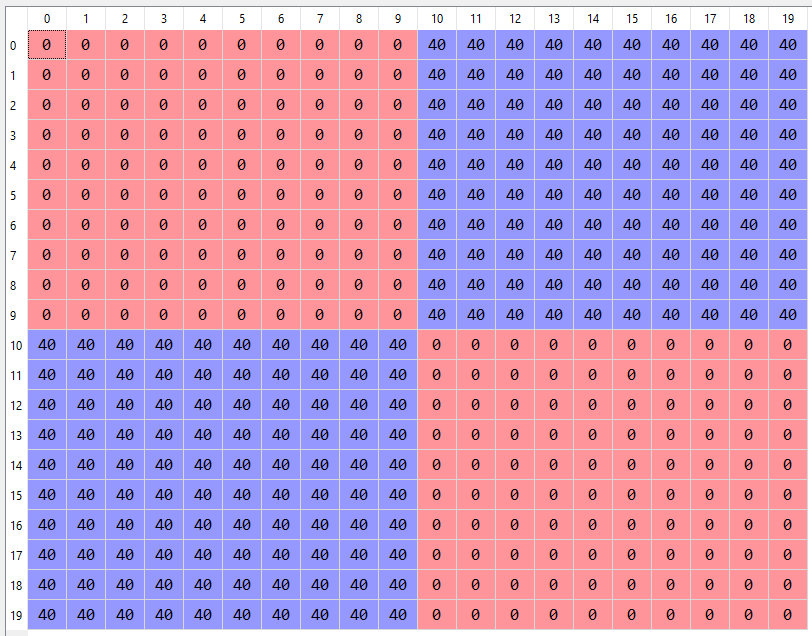
\includegraphics[width = 1\textwidth]{i.png}
\caption{Input image}
\label{i}
\end{figure}

After applying Prewitt mask:
\begin{figure}[H]
\centering
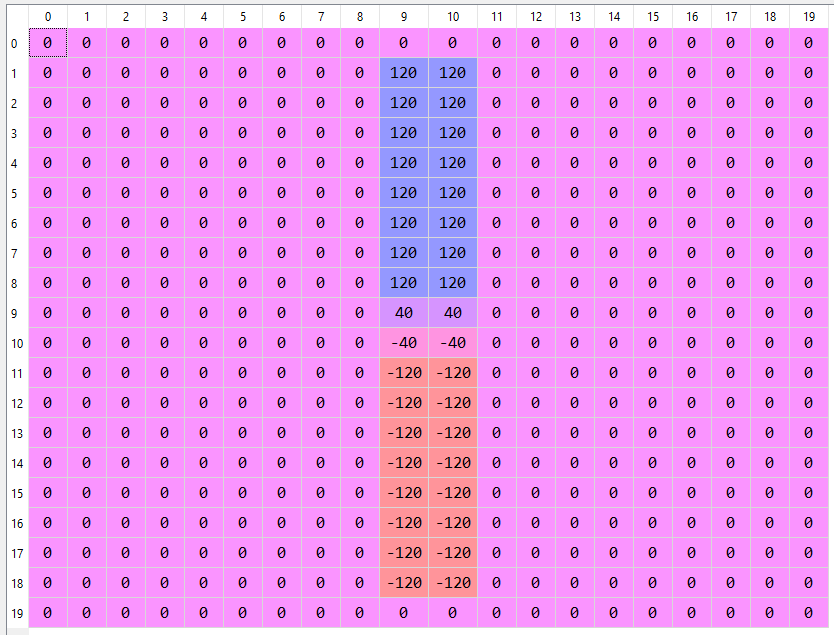
\includegraphics[width = 0.8\textwidth]{ex.png}
\caption{Ex}
\label{ex}
\end{figure}
\begin{figure}[H]
\centering
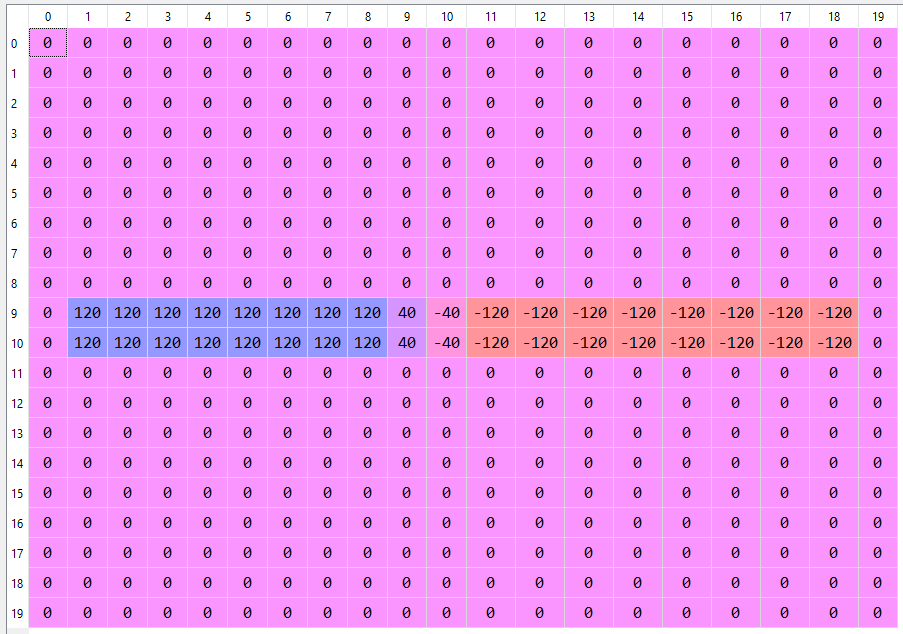
\includegraphics[width = 0.8\textwidth]{ey.png}
\caption{Ey}
\label{ey}
\end{figure}
\noindent Since we consider a neighborhood of $7\times7$, the border of width 3 can also be disregarded, and thus we only calculated those valid pixels of the $14\times 14$ matrix in the center. For each pixel, its $C$ matrix can be given by 
\begin{equation*}
C = \left[ \begin{array}{cc}
\sum E_x^2 & \sum E_xE_y\\
\sum E_xE_y & \sum E_y^2
\end{array} \right]
\end{equation*}
For each $C$ matrix, we can calculate its eigenvalues $\lambda_1$,  $\lambda_2$, and select $min\{\lambda_1, \lambda_2\}$ to form a minimum eigenvalue matrix as shown in Fig \ref{eigen}
\begin{figure}[H]
\centering
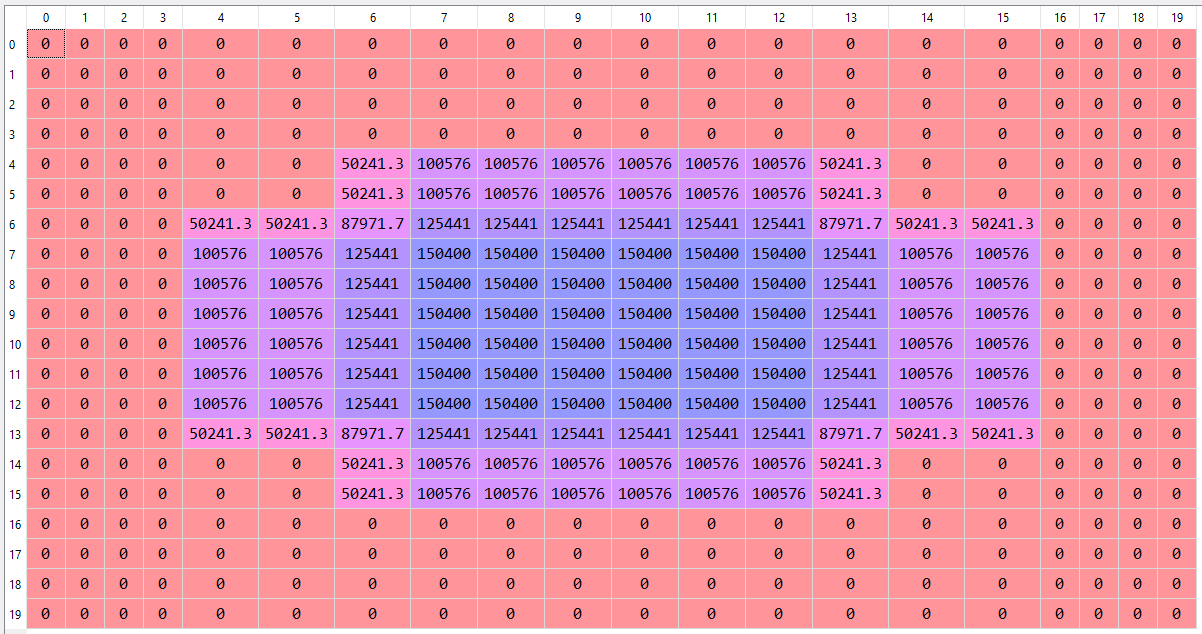
\includegraphics[width = 1\textwidth]{eigen.png}
\caption{Minimum Eigenvalue Matrix}
\label{eigen}
\end{figure}
\noindent The corner has a high likelihood to be located within the $6\times6$ region in the center.
%%---------------------------------------------------------------
%% Question 4
%%---------------------------------------------------------------
\section{Solution:}
Using the normal equation

\begin{table*}[h]
%\caption{\label{table_1} }
\centering
\begin{tabular}{|c|c|c|}
\hline
\textbf{Side}&$\rho$& \textbf{$\Theta$}\\
\hline
AB & 2 & 0\\
BC & 2 & 90 \\
CA & $\sqrt{2}$ & 45\\
\hline
\end{tabular}
\end{table*}
\noindent After modification:\\
\begin{table*}[h]
%\caption{\label{table_1} }
\centering
\begin{tabular}{|c|c|c|}
\hline
\textbf{Side}&$\rho$& \textbf{$\Theta$}\\
\hline
AB & 4 & 90\\
BC & -4 & 0 \\
CA & -2 & -45\\
\hline
\end{tabular}
\end{table*}
\vfill
\clearpage

\noindent \\
As shown in Fig \ref{area}, the area of the modified object is $36 - 16\sqrt{2}$.
\begin{figure}[H]
\centering
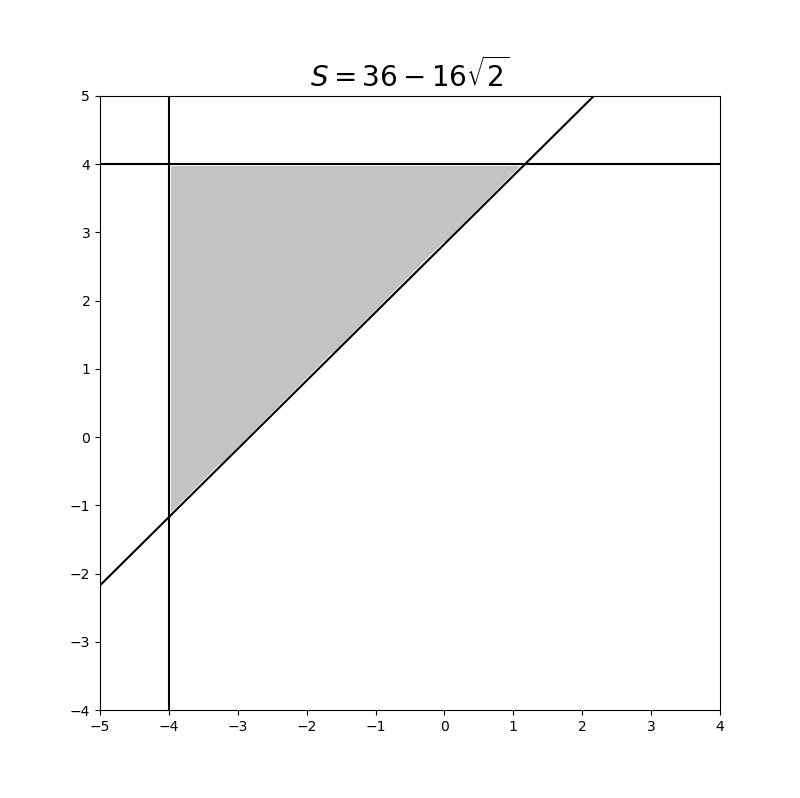
\includegraphics[width = 0.6\textwidth]{area.png}
\caption{Area of the modified object}
\label{area}
\end{figure}
%%---------------------------------------------------------------
%% Question 5
%%---------------------------------------------------------------
\section{Solution:}
(a) The line equations in image space can be given by:
\begin{equation*}
\begin{aligned}
&AB: y=3\\
&BC: x=3\\
&CD: y=2-\frac{x}{\sqrt{3}}\\
&DA: y=x+1
\end{aligned}
\end{equation*}
And the coordinates of the four vertices are:
\begin{equation*}
\begin{aligned}
&A (2, 3)\\
&B (3, 3)\\
&C  (3, 2-\sqrt{3})\\
&D (\frac{\sqrt{3}}{\sqrt{3+1}}, \frac{2\sqrt{3}+1}{\sqrt{3}+1})
\end{aligned}
\end{equation*}
Image is shown in Fig \ref{polygon}.
\begin{figure}[H]
\centering
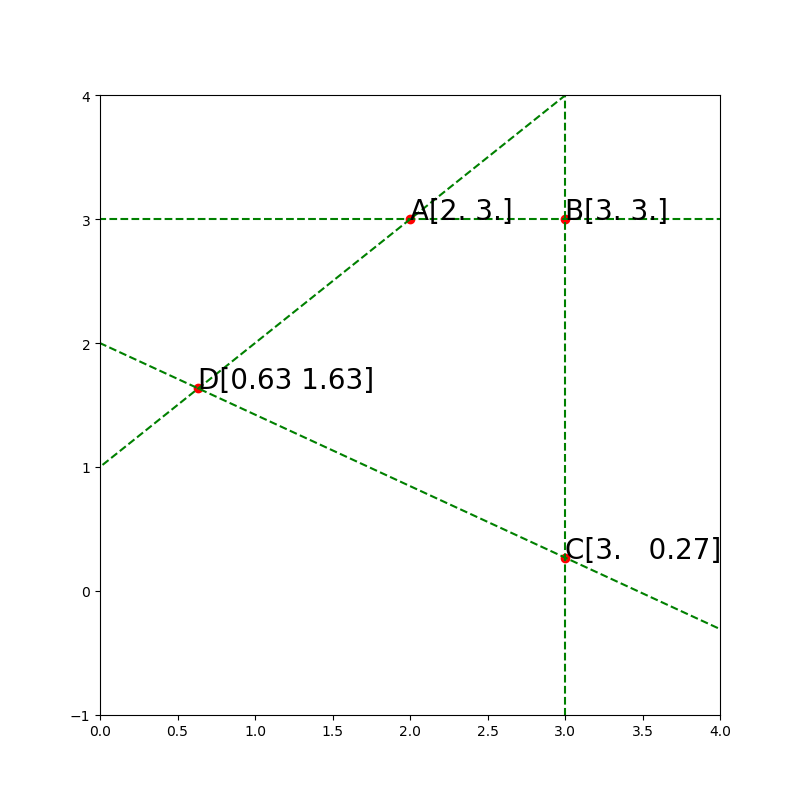
\includegraphics[width = 0.6\textwidth]{p5.png}
\caption{The polygon}
\label{polygon}
\end{figure}

(b) After rotating, the radius $\rho$ keeps the same, and \textbf{$\Theta$} increases $30$ degrees.
\begin{table*}[h]
%\caption{\label{table_1} }
\centering
\begin{tabular}{|c|c|c|}
\hline
\textbf{Side}&$\rho$& \textbf{$\Theta$}\\
\hline
AB & -3 & -30\\
BC & 3 & 30 \\
CD & $\sqrt{3}$ & 90\\
DA & $-\sqrt{2}/2$ & -15\\
\hline
\end{tabular}
\end{table*}

%%---------------------------------------------------------------
%% Question 6
%%---------------------------------------------------------------
\section{Solution:}
Consider the residual value for every data point:
\begin{equation*}
r_i = Ax_i + By_i+C - g_i  \sim N(0, \sigma^2)
\end{equation*}
For the given two regions:
\begin{equation*}
r_{1}, r_{1}, ..., r_{m} \in R_1 \sim N(0, \sigma_1^2)
\end{equation*}
\begin{equation*}
r_{m+1}, r_{m+2}, ..., r_{m+n} \in R_2\sim N(0, \sigma_2^2)
\end{equation*}
Two possible HYPOTHESES:\\
\textbf{$H_0$}: Both regions belong to the same object and the residual values have distribution $N(0, \sigma_0^2)$.\\
\textbf{$H_1$}: Each region belongs to a different object and their residual values have distributions $N(0, \sigma_1^2)$ and $N(0, \sigma_2^2)$.\\

\vfill
\clearpage

\noindent Estimated $\sigma_0^2$:
\begin{equation*}
\begin{aligned}
\sigma_0^2&=\frac{1}{m+n}\sum_{r_i\in R_1\cup R_2}r_i^2\\
& = \frac{1}{m+n}\left (\sum_{r_i\in R_1}r_i^2+\sum_{r_i\in R_2}r_i^2 \right)\\
&=\frac{m\sigma_1^2+n\sigma_1^2}{m+n}
\end{aligned}
\end{equation*}
Compute the probability of independently drawing $r_1, r_2, ..., r_{m+n}$ with distribution $N(0, \sigma_0^2)$:

\begin{equation*}
\begin{aligned}
P\left ( r_1, r_2,...,r_{m+n}|H_0 \right )&=\prod^{m+n}_{i=1}P(r_i|H_0)\\
&=\prod^{m+n}_{i=1}\frac{1}{\sqrt{2\pi}\sigma_0}e^{-r_i^2/2\sigma_0^2}\\
&=\frac{1}{(\sqrt{2\pi}\sigma_0)^{m+n}}e^{-(m+n)/2}
\end{aligned}
\end{equation*}
Similarly,
\begin{equation*}
P\left ( r_1,...,r_m|H_1 \right )=\prod^m_{i=1}P(r_i|H_1)
=\prod^m_{i=1}\frac{1}{\sqrt{2\pi}\sigma_1}e^{-r_i^2/2\sigma_1^2}
=\frac{1}{(\sqrt{2\pi}\sigma_1)^m}e^{-m/2}
\end{equation*}
\begin{equation*}
P\left ( r_{m+1}, ...,r_n|H_1 \right )=\prod^{m+n}_{i=m+1}P(r_i|H_1)
=\prod^{m+n}_{i=m+1}\frac{1}{\sqrt{2\pi}\sigma_2}e^{-r_i^2/2\sigma_2^2}
=\frac{1}{(\sqrt{2\pi}\sigma_2)^n}e^{-n/2}
\end{equation*}
\begin{equation*}
P\left (r_1, r_2,...,r_{m+n}|H_1 \right )=\frac{1}{(\sqrt{2\pi})^{m+n}\sigma_1^m\sigma_2^n}e^{-(m+n)/2}
\end{equation*}
\begin{equation*}
L = \frac{P\left (r_1, r_2,...,r_{m+n}|H_1 \right)}{P\left (r_1, r_2,...,r_{m+n}|H_0 \right )}=\frac{\sigma_0^{m+n}}{\sigma_1^m\sigma_2^n}
=\frac{\left ( \frac{m\sigma_1^2+n\sigma_1^2}{m+n}\right )^{m+n}}{\sigma_1^m\sigma_2^n}
\end{equation*}
If $L < 1$, $H_0$ is more likely than $H_1$, and the regions are to be merged.
%%---------------------------------------------------------------
%% Question 7
%%---------------------------------------------------------------
\section{Solution:}
(a) Applying mean shift to find the window peak: \\
\textbf{Iteration 1}:
\begin{equation*}
r = 2,\ x_0 = 4 \longrightarrow 2\leq y\leq6
\end{equation*}
\begin{equation*}
\mu = \frac{2\times2+3\times3+4\times2+5\times1+6\times1}{2+3+2+1+1} - 4 = -\frac{4}{9}
\end{equation*}
\textbf{Iteration 2}:
\begin{equation*}
r = 2,\ x_1 = \frac{32}{9} \longrightarrow 2\leq y\leq5
\end{equation*}
\begin{equation*}
\mu = \frac{2\times2+3\times3+4\times2+5\times1}{2+3+2+1} - \frac{32}{9} = -\frac{11}{36}
\end{equation*}
\textbf{Iteration 3}:
\begin{equation*}
r = 2,\ x_2 = \frac{13}{4} \longrightarrow 2\leq y\leq5
\end{equation*}
\begin{equation*}
\mu = \frac{2\times2+3\times3+4\times2+5\times1}{2+3+2+1} - \frac{13}{4} = 0
\end{equation*}
After the 3rd iteration, the mode converges at $13/4$.\\
(b) With approximation $a = 13/4$, the fitting error
\begin{equation*}
\begin{aligned}
MSE &= \frac{1}{N}\sum_{i=1}^N (g_i-a)^2\times n_i \\
&= \frac{(1-\frac{13}{4})^2 \times 1 + (2-\frac{13}{4})^2 \times 2 +(3-\frac{13}{4})^2 \times 3 +(4-\frac{13}{4})^2 \times 2 +(5-\frac{13}{4})^2 \times 1 + (6-\frac{13}{4})^2 \times 1}{1+2+3+2+1+1}\\
&= \frac{277}{16\times10} = \frac{277}{160}
\end{aligned}
\end{equation*}
The mean squared error is $277/160$.\\
(c) $\hat{\mu} = 13/4$, $\hat{\sigma}^2 = 277/160$
\begin{equation*}
\begin{aligned}
L_0 &= P(g_1g_2...g_N|\hat{\mu}\hat{\sigma})\\
& = \prod^N_{i=1}P(g_i|\hat{\mu}\hat{\sigma})\\
& = \prod^N_{i=1} \frac{1}{\sqrt{2\pi}\hat{\sigma}} e^{-(g_i-\hat{\mu})^2/2\hat{\sigma}^2}\\
& = \frac{1}{(\sqrt{2\pi}\hat{\sigma})^N}e^{-\sum_{i=1}^N(g_i-\hat{\mu})^2/2\hat{\sigma}^2}\\
& = \frac{1}{(\sqrt{2\pi}\hat{\sigma})^N}e^{-N/2}\\
& = \left (\frac{160}{2\pi\times277} \right )^5e^{-5}\\
& = 4.4\times 10^{-8}
\end{aligned}
\end{equation*}


\end{document}
